\documentclass[masters,draft]{UTPAthesis}
%\documentclass[masters,final]{UTPAthesis}


%% Load your packages below.
%% Make hyperref and showkeys come at the end of your loaded packages
%% to make sure they are not over-written.  They redefine many
%% standard LaTeX commands
\usepackage{booktabs} % for better tables
\usepackage[colorlinks=false]{hyperref}  % for urls
\usepackage{showkeys}  % shows labels during draft mode


% Insert your name here
\Author{John Q. Citizen}
\Major{Mathematics}


% Insert your graduation date here
\Year{2014}
\Month{May}


% Insert the title of your thesis here.
% If you have a long title, split it between multiple lines using the \\ command
 \Title{Titles Should Not Exceed Six Inches on One Line\\
   and In The Inverted Pyramid Format\\
   When Additional Lines Are Needed
}


% Insert your research advisor and his title here
 \Advisor{Dr. Leonhard Euler}
 \AdvisorTitle{Chair of Committee}


%% Insert the members of your committee here
 \MemberA{Dr. Carl Friedrich Gauss}
 \MemberB{Dr. G. F. Bernhard Riemann}
 \MemberC{}
 \MemberD{}


% Insert the text of your abstract here
 \Abstract{The abstract is double spaced, including the heading, which begins
two inches down from the top of the page. Note that the abstract title is
underlined and that any italicized words are not underlined (in order to
indicate italics).  If an abstract title contains scientific terminology
requiring italics, such terminology should be treated in the same manner. Do
not use italic print in the abstract title.  Right and left margins are the
same as for the body of the thesis. Note that the author's name and thesis
title must be identical on the title page, the approval page, and the
abstract heading. The date of graduation is the same as that shown on the
title page. The number of titles is the number of items in the bibliography
or reference list. Word limits are 150 for master's theses and 350 for
doctoral dissertations. Count numbers as words, hyphenated words as two
words. Acronyms, abbreviations, and initials as words. }


% You can dedicate your paper here
\Dedication{%
    Dedication should be simple, in good taste, and fit on one page.
  }

% Acknowledge those who helped and supported you here.
  \Acknowledgments{%
    Acknowledgements should be simple, in good taste, and fit on one page.
  }

% Insert your biographical sketch here.
  \BiographicalSketch{%
    A brief biographical sketch of the student is required as part of each thesis.
  }


\begin{document}

 % This starts page counting in Roman numerals
 \frontmatter

 % This command makes the formal preliminary pages.
 % You can comment it out during the drafting process if you want to save paper.
 \makepreliminarypages

 % These insert a table of contents, list of tables, and list of figures.
 \tableofcontents
 \listoftables
 \listoffigures

 % This starts regular page counting in Arabic numerals
 \mainmatter


% OK. Everything is set up. Insert your thesis below.
% It's a good idea to split your thesis up into different files and use
% the \input command
\chapter{Introduction}

In Synthetic Aperture Radar (SAR) imaging, radar antennas are mounted on an airborne or spaceborne platform. The scene to be imaged is illuminated by electromagnetic waves transmitted from an antenna. The goal is to extract information of the scene from the measurements taken of the scattered waves.

\section{Blah Blah}


Many of the principles of SAR imaging are applicable to other fields such as
acoustics, geophysics, and medical imaging. In particular, it has been shown
that spotlight-mode SAR can be described as a tomographic reconstruction problem
and can be analyzed using the projection slice theorem from computer-aided
tomography\cite{Garza:2011fk}

\begin{equation}\label{eq:einstein}
	e = mc^{2}
\end{equation}



\begin{figure}
  \centering
  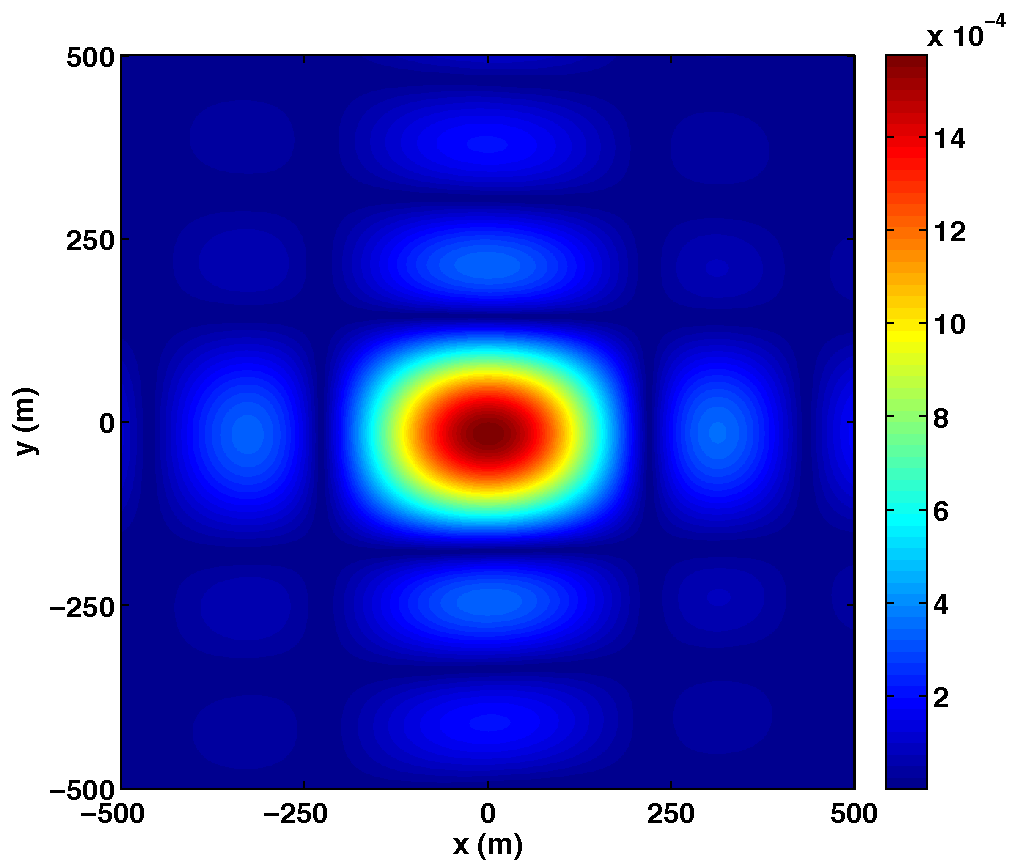
\includegraphics[scale=0.5]{figures/beamfootprint}
  \caption[Colorful Picture]{This is a colorful picture.}
  \label{fig:flyover}
\end{figure}




%  Uncomment the following line for appendixes
%\appendix


% This makes the bibliography.
% Enter your references in the BibTex file "references.bib"
% You can find bibtex info from Google Scholar.
\bibliographystyle{siam}
\bibliography{references}


% This inserts your Biographical Sketch
\biographypage

\end{document}
